%-------
% Notes
%   ~ADD       : Add the following.
%   ~REFERENCE : Reference the following paper/authors.
%   ~FIND      : Find a paper regarding the following.
%   ~CHECK     : Check that the following is met.
%   ~READ      : Read through the following paper/authors.
%   ~MENTION   : Mention the following.
%   ~AMMEND    : Make a change to the following.
%   ~IDEA      : Suggestion for later in the project.

\documentclass{UoYCSproject}
\usepackage{geometry}

% -----------
% Tikz Setup 
\usepackage{tikz}
\usetikzlibrary{ matrix,      % For easy node positioning
                 fit,         % For easily fitting nodes inside another one
                 arrows,
                 positioning, % For easy node-relative placements
               }
\tikzstyle{edge} = [->, bend left]
\tikzstyle{edge'} = [->, bend right]
\tikzstyle{vertex} = [circle, minimum width=0.5cm, text centered, draw=black]
\tikzstyle{mark_grey} = [fill=grey]
\tikzstyle{graph_small} = [rectangle, draw=black, inner sep=0.5cm]
\tikzstyle{graph} = [rectangle, draw=black, inner sep=1cm]
\tikzstyle{rule} = [rectangle, inner sep=1cm]
\tikzstyle{derivation} = [-implies, double, thick]

% ---------------
% Listings Setup
\usepackage{listings}
\renewcommand{\lstlistingname}{Program Code}

\author{Huw Taylor}
\title{Tracing GP2 Execution} %TODO ~AMMEND: is 'Execution' needed? Maybe just Tracing GP2?
\date{\today}
\supervisor{Dr. Detlef Plump}
\MEng
%TODO ~CHECK: The word/page counts are up to date.
\wordcount{-1}
\pagecount{-1}
% ~16000 words (55 pages) total
\abstract{
% ~66 words

}
\acknowledgements{
I would like to thank Christopher Bak for his support throughout the project. His advice on the workings of the GP2 compiler has been invaluable.
% Detlef?
}

\begin{document}

\maketitle
\tableofcontents
% \listoffigures

\chapter{Introduction}
% ~1333 words
\section{Motivation}
%TODO ~ADD: some references for this stuff. I have them, just chuck in citations to papers I already got.
GP is a graph programming language. It was developed to provide a language that is expressive enough to solve complex graph problems, while also having a simple enough syntax to allow for formal reasoning. Graphs and graph transformations have previously implemented in low-level languages, like C. This meant that it was more difficult to understand, verify, and implement \cite{gp_lang}. GP at its core has four commands that nevertheless allows every computable function on graphs to be implemented \cite{gp1}. These commands are a single application of a rule, sequential composition, loops, and branching. Loops are implemented in a run-for-as-long-as-possible style.

GP2, the second iteration of GP, builds upon the first. It adds a few new features, and some syntactic sugar \cite{gp2_design}. Also, the design of GP2 was slightly modified to enable a higher level of performance. A compiler was produced by the University of York for GP2. The compiler generates C code from a high level representation of a graph program in GP2. This has the advantage of being able to reason about graphs and graph programming using GP2, but allows for the low-level, high-performance that C allows for.

The University of York has also produced a graphical editor for creating graphs and graph programs. The editor depends on the compiler to execute the program on the host graph, thereby producing the resultant graph. It displays the graphs, and has a graphical user interface for creating graphs, rules and programs.

Currently, the compiler generates the code to run the entire program on the given host graph. It generates code for each rule and a main program file which makes use of the rules' code. After compilation, the C code implementation of the graph program can be run on the graph, and the resultant graph is saved in the given output directory.

If the graphical editor is being used, the user can graphically create the host graph, and the rules for the program within it, and can run their program on their host graph, and the editor will show them the resultant graph.

The aim of this project is to show the execution of the program, that is, the intermediate steps that result in the final output graph. This will allow users to see the process, which enables the correctness of the program to be ensured. It will also give people using these tools, who may not have a complete understanding of how graph programs work in general, or who aren't sure about their specific program's execution in particular, the opportunity to see the process with a finer granularity.

This tracing of graph programs will sit atop the existing GP2 implementation and be completely optional for any users. It will allow for deeper and more powerful visualisations of graph programs and their execution.
%

\section{Ethics}
The project discussed has very few ethical considerations. It is not related to defence and there are no safety or security concerns. No humans or animals are involved in its development.

\chapter{Literature Review}
% ~4000 words
%TODO ~CHECK: Shows that you know what is happening in your field 
%TODO ~CHECK: Justifies why your work is interesting or important 
%TODO ~CHECK: establishes the theoretical framework/context for your work 
%TODO ~CHECK: defends your choice of methodology 
%TODO ~CHECK: avoids repeating previous researchers’ mistakes
\section{Graph Programming}

\subsection{Graph Transformations}
A graph is a visual way of representing data and relationships. The formal definition is a set of vertices (nodes) \emph{V}, a set of edges \emph{E}, and a set of labels \emph{L}. Additionally \emph{source} and \emph{target} functions associate edges with nodes, and a \emph{label} function, which assigns labels to edges and nodes.
Graph theory is said to go back as far as the 1730s, with The K{\"o}nigsberg Bridge problem being regarded as the topic for the first paper on graph theory ever written \cite{grathe_origin}. 

The mathematical theory of Graph Transformation allows the transformation of graphs by way of rules. Rules are applied to graphs. They include a LHS (Left-Hand Side) graph, and RHS (Right-Hand Side) graph and an interface graph, which connects nodes in the LHS to nodes in the RHS. There is a convention that if the interface graph is ommited then it is inferred that it comprises the common labelled nodes in both the LHS and RHS.

Rules can either use a single-pushout or a double-pushout approach. In GP, graph transformations use the double-pushout with relabelling \cite[p. 100]{gp1}. Matches of rules must be injective morphisms and are only vaild if they don't result in \emph{dangling edges}, that is, edges with one or more ends not attactched to a node. The interface graph of a rule may be partially labelled, but all other graphs must be totally labelled. A partially labelled graph is %TODO definition of partially labelled graphs
, whereas a totally labelled graph is %TODO definiton of totally labelled graph

Figure \ref{fig:simple_rule} shows a simple rule that, given a non-empty host graph, creates a transitive graph, where every node with a directed path to another has a direct edge going to it. A directed path between two nodes \emph{A} and \emph{B} exists either if there is an outgoing edge from \emph{A} to \emph{B}, or for any of the nodes that have an incoming edge from \emph{A}, there is a directed path from it to \emph{B}.
Figure \ref{fig:simple_rule_sans_k} shows the same rule without its interface graph.

\begin{figure}
\label{fig:simple_rule}
\centering
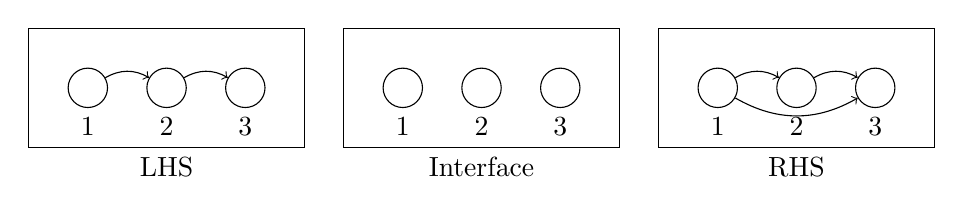
\begin{tikzpicture}[scale=2]
  \node (n1) [vertex, label=below:{1}] at (0, 0) {};
  \node (n2) [vertex, label=below:{2}] at (0.5, 0) {};
  \node (n3) [vertex, label=below:{3}] at (1, 0) {};
  \path [edge] (n1) edge node {} (n2);
  \path [edge] (n2) edge node {} (n3);
  \node (l) [graph_small, fit={(n1) (n2) (n3)}, label=below:{LHS}] {};
  
  \node (n4) [vertex, label=below:{1}] at (2, 0) {};
  \node (n5) [vertex, label=below:{2}] at (2.5, 0) {};
  \node (n6) [vertex, label=below:{3}] at (3, 0) {};
  \node (k) [graph_small, fit={(n4) (n5) (n6)}, label=below:{Interface}] {};
  
  \node (n7) [vertex, label=below:{1}] at (4, 0) {};
  \node (n8) [vertex, label=below:{2}] at (4.5, 0) {};
  \node (n9) [vertex, label=below:{3}] at (5, 0) {};
  \path [edge] (n7) edge node {} (n8);
  \path [edge] (n8) edge node {} (n9);
  \path [edge'] (n7) edge node {} (n9);
  \node (r) [graph_small, fit={(n7) (n8) (n9)}, label=below:{RHS}] {};
\end{tikzpicture}
\caption{Rule Example}
\end{figure}

\begin{figure}
\label{fig:simple_rule_sans_k}
\centering
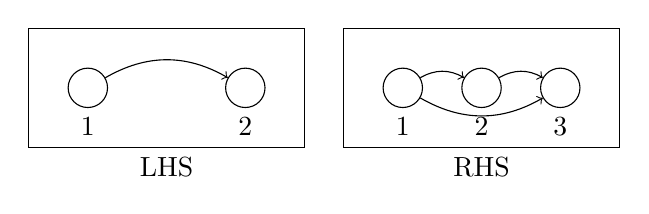
\begin{tikzpicture}[scale=2]
  \node (n1) [vertex, label=below:{1}] at (0, 0) {};
  \node (n2) [vertex, label=below:{2}] at (1, 0) {};
  \path [edge] (n1) edge node {} (n2);
  \node (l) [graph_small, fit={(n1) (n2)}, label=below:{LHS}] {};
  
  \node (n7) [vertex, label=below:{1}] at (2, 0) {};
  \node (n8) [vertex, label=below:{2}] at (2.5, 0) {};
  \node (n9) [vertex, label=below:{3}] at (3, 0) {};
  \path [edge] (n7) edge node {} (n8);
  \path [edge] (n8) edge node {} (n9);
  \path [edge'] (n7) edge node {} (n9);
  \node (r) [graph_small, fit={(n7) (n8) (n9)}, label=below:{RHS}] {};
\end{tikzpicture}
\caption{Rule Example without Interface Graph}
\end{figure}

Rules are applied using % morphisms? Explain the morphism.

%TODO ~ADD: "construction of rule application" how a rule works. 
% Find the match
	% LHS morphism onto graph?
% apply the rule. 
	% pushouts (double/single)
	% label preserving, but can change them

%TODO illustrate the process of a rule's application
\begin{figure}
\label{fig:simple_rule}
\centering
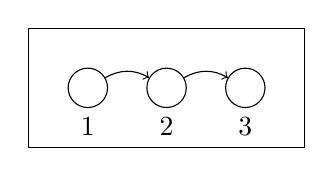
\begin{tikzpicture}[scale=2]
  \node (n1) [vertex, label=below:{1}] at (0, 0) {};
  \node (n2) [vertex, label=below:{2}] at (0.5, 0) {};
  \node (n3) [vertex, label=below:{3}] at (1, 0) {};
  \path [edge] (n1) edge node {} (n2);
  \path [edge] (n2) edge node {} (n3);
  \node (l) [graph_small, fit={(n1) (n2) (n3)}, label=below:{}] {};
\end{tikzpicture}
\caption{Rule Example}
\end{figure}

\subsection{Graph Programs}
The University of York has developed a graph programming language \emph{"GP1"} \cite{gp1}, and has developed a new implementation \emph{"GP2"}. The goal of both of these has been to write programs that manipulate graphs in terms of the graphs, rather than in general purpose languages like C or Java. 

Graph programming (GP) allows the application of programs to graphs. A program is made up of rules and rudimentary control structures, such as conditions, and loops. The rules are executed non-deterministically on a graph, known as the \emph{host graph}. The resulting graph is known as the \emph{result graph}. A simple program could just be the continued application of a single rule.
%TODO ~ADD, ~REFERENCE: Greg Manning Paper

%TODO ~ADD describe constants of the language
% Graph programs have macros, and rules, and if statements, try statements, and loops, and non-deterministic choosing between macros/rules.
% The syntax is XYZ
% Chris's Paper, page 41 has the abstract syntax of GP2 programs. Steal it! Steal iiiit!!

%TODO ~ADD: more stuff about GP (page 18 on https://www.cs.york.ac.uk/ftpdir/reports/2007/YCST/15/YCST-2007-15.pdf (gp_lang) and page 1 on https://www.cs.york.ac.uk/plasma/publications/pdf/Plump.CAI.09.pdf (gp1))

%TODO ~AMMEND: Make the code portion of this picture truetype
%TODO ~AMMEND: Look at the GRAT slides and use the shortest distance program there (which uses GP2 stuff, rather than GP1 stuff) http://www-module.cs.york.ac.uk/grat/Lectures/VII.pdf page 35
\begin{figure}
\label{fig:simple_program}
\centering
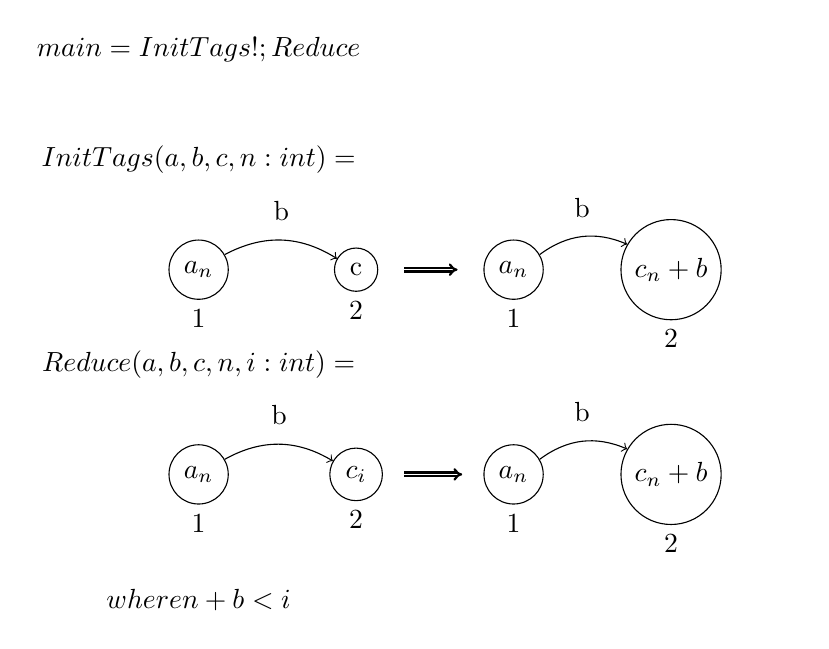
\begin{tikzpicture}[scale=2]
  \node (code) at (0, 3.5) {$main = InitTags!; Reduce$};
  \node (rule_1) at (0, 2.8) {$InitTags(a,b,c,n : int) = $};

  \node (n1) [vertex, label=below:{1}] at (0, 2.1) {$a_n$};
  \node (n2) [vertex, label=below:{2}] at (1, 2.1) {c};
  \path [edge] (n1) edge node[label=above:{b}] {} (n2);
  \node (r1_l) [rule, fit={(n1) (n2)}] {};
  
  \node (n3) [vertex, label=below:{1}] at (2, 2.1) {$a_n$};
  \node (n4) [vertex, label=below:{2}] at (3, 2.1) {$c_n+b$};
  \path [edge] (n3) edge node[label=above:{b}] {} (n4);
  \node (r1_r) [rule, fit={(n3) (n4)}] {};
  
  \draw[derivation] (r1_r) -> (r1_l); % dafuq is this backwards bullshit?
  
  \node (rule_2) at (0, 1.5) {$Reduce(a,b,c,n,i : int) = $};  
  
  \node (n5) [vertex, label=below:{1}] at (0, 0.8) {$a_n$};
  \node (n6) [vertex, label=below:{2}] at (1, 0.8) {$c_i$};
  \path [edge] (n5) edge node[label=above:{b}] {} (n6);
  \node (r2_l) [rule, fit={(n5) (n6)}] {};
  
  \node (n7) [vertex, label=below:{1}] at (2, 0.8) {$a_n$};
  \node (n8) [vertex, label=below:{2}] at (3, 0.8) {$c_n+b$};
  \path [edge] (n7) edge node[label=above:{b}] {} (n8);
  \node (r2_r) [rule, fit={(n7) (n8)}] {};
  
  \draw[derivation] (r2_r) -> (r2_l); % ~EDIT: Maybe use the deriviation tikz thing defined at the top.
  \node (rule_2_condition) at (0, 0) {$where n+b < i$};  

\end{tikzpicture}
\caption{Simple Dijkstra Program Example}
\end{figure}


The program \ref{fig:simple_program} finds the shortest path to each node, using Dijkstra's algorithm for pathfinding. Running it on the host graph will give the intermediary graphs shown in \ref{fig:simple_program_example}.

%TODO ~AMMEND: Use the ammended program to recreated the process. Also, add some more steps.
\newgeometry{left=1cm,bottom=0.1cm}

\begin{figure}
\label{fig:simple_program_example}
\centering
%TODO ~CHECK: Make sure this displays how it should.
%TODO ~ADD: Colour to illustrate changes?
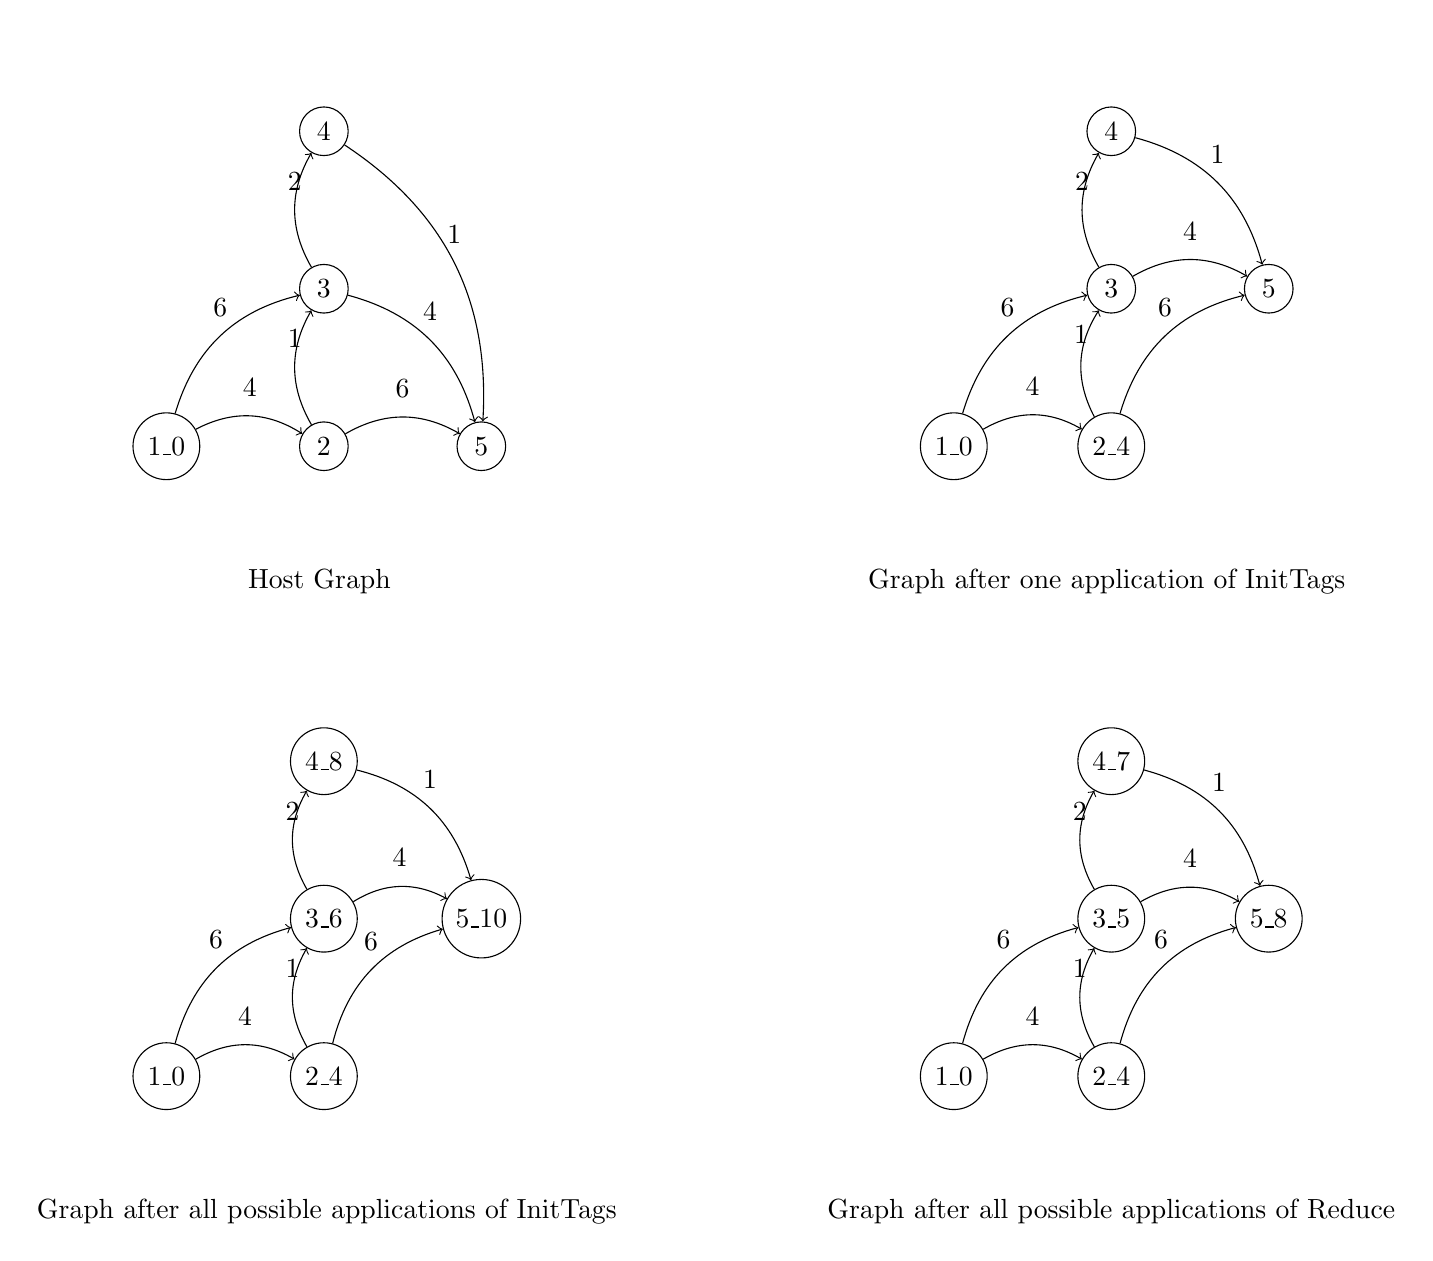
\begin{tikzpicture}[scale=2]
  \node (n1_1) [vertex] at (0, 4) {$1\_0$};
  \node (n1_2) [vertex] at (1, 4) {2};
  \node (n1_3) [vertex] at (1, 5) {3};
  \node (n1_4) [vertex] at (1, 6) {4};
  \node (n1_5) [vertex] at (2, 4) {5};
  \path [edge] (n1_1) edge node[label=above:{4}] {} (n1_2);
  \path [edge] (n1_1) edge node[label=above:{6}] {} (n1_3);
  \path [edge] (n1_2) edge node[label=above:{1}] {} (n1_3);
  \path [edge] (n1_3) edge node[label=above:{2}] {} (n1_4);
  \path [edge] (n1_2) edge node[label=above:{6}] {} (n1_5);
  \path [edge] (n1_3) edge node[label=above:{4}] {} (n1_5);
  \path [edge] (n1_4) edge node[label=above:{1}] {} (n1_5);
  \node (g0) [rule, fit={(n1_1) (n1_2) (n1_3) (n1_4) (n1_5)}, label=below:{Host Graph}] {};
  
  \node (n2_1) [vertex] at (5, 4) {$1\_0$}; % probably have to change these coordinates.
  \node (n2_2) [vertex] at (6, 4) {$2\_4$};
  \node (n2_3) [vertex] at (6, 5) {3};
  \node (n2_4) [vertex] at (6, 6) {4};
  \node (n2_5) [vertex] at (7, 5) {5};
  \path [edge] (n2_1) edge node[label=above:{4}] {} (n2_2);
  \path [edge] (n2_1) edge node[label=above:{6}] {} (n2_3);
  \path [edge] (n2_2) edge node[label=above:{1}] {} (n2_3);
  \path [edge] (n2_3) edge node[label=above:{2}] {} (n2_4);
  \path [edge] (n2_2) edge node[label=above:{6}] {} (n2_5);
  \path [edge] (n2_3) edge node[label=above:{4}] {} (n2_5);
  \path [edge] (n2_4) edge node[label=above:{1}] {} (n2_5);
  \node (g1) [rule, fit={(n2_1) (n2_2) (n2_3) (n2_4) (n2_5)}, label=below:{Graph after one application of InitTags}] {};
  
  \node (n3_1) [vertex] at (0, 0) {$1\_0$}; % probably have to change these coordinates.
  \node (n3_2) [vertex] at (1, 0) {$2\_4$};
  \node (n3_3) [vertex] at (1, 1) {$3\_6$};
  \node (n3_4) [vertex] at (1, 2) {$4\_8$};
  \node (n3_5) [vertex] at (2, 1) {$5\_10$};
  \path [edge] (n3_1) edge node[label=above:{4}] {} (n3_2);
  \path [edge] (n3_1) edge node[label=above:{6}] {} (n3_3);
  \path [edge] (n3_2) edge node[label=above:{1}] {} (n3_3);
  \path [edge] (n3_3) edge node[label=above:{2}] {} (n3_4);
  \path [edge] (n3_2) edge node[label=above:{6}] {} (n3_5);
  \path [edge] (n3_3) edge node[label=above:{4}] {} (n3_5);
  \path [edge] (n3_4) edge node[label=above:{1}] {} (n3_5);
  \node (gx) [rule, fit={(n3_1) (n3_2) (n3_3) (n3_4) (n3_5)}, label=below:{Graph after all possible applications of InitTags}] {}; 
  
  \node (n4_1) [vertex] at (5, 0) {$1\_0$}; % probably have to change these coordinates.
  \node (n4_2) [vertex] at (6, 0) {$2\_4$};
  \node (n4_3) [vertex] at (6, 1) {$3\_5$};
  \node (n4_4) [vertex] at (6, 2) {$4\_7$};
  \node (n4_5) [vertex] at (7, 1) {$5\_8$};
  \path [edge] (n4_1) edge node[label=above:{4}] {} (n4_2);
  \path [edge] (n4_1) edge node[label=above:{6}] {} (n4_3);
  \path [edge] (n4_2) edge node[label=above:{1}] {} (n4_3);
  \path [edge] (n4_3) edge node[label=above:{2}] {} (n4_4);
  \path [edge] (n4_2) edge node[label=above:{6}] {} (n4_5);
  \path [edge] (n4_3) edge node[label=above:{4}] {} (n4_5);
  \path [edge] (n4_4) edge node[label=above:{1}] {} (n4_5);
  \node (gn) [rule, fit={(n4_1) (n4_2) (n4_3) (n4_4) (n4_5)}, label=below:{Graph after all possible applications of Reduce}] {}; 
  
\end{tikzpicture}
\caption{Simple Dijkstra Program Example}
\end{figure}

\restoregeometry

\section{GP2 Compiler}
Instead of using an abstract machine as GP1 did, the GP2 compiler generates C code directly \cite{chris_compiler}, which removes the reliance on specific abstract machine compilers and data formats for graphs and graph programs. It means that any C compiler can be used to generate the program code. It also attempts to standardise and document the format of graphs and programs that it takes. This means that tools to generate graphs either graphically or programmatically can be created without reducing modularity or creating complexity and interdependance between the components of the system \cite{gp2_ide}.

GP2 adds to GP the marking of nodes with a colour, or a special 'any' colour; additional conditions that can be checked against in a rule's schema, including the in-degree and out-degree of an edge, and whether there exists an edge between two nodes; and an additional branching mechanism: a try-then-else. In try-then-else and if-then-else branching, the condition is a set of rules schemata, and almost always alters the graph. If-then-else branching uses the graph before the 'if' condition is evaluated, and any changes are made, in the 'then' branch. In contrast, the try-then-else uses the \emph{result} of the 'try' condition in the 'then' branch. In both, the 'else' branch uses the graph before the condition is checked against \cite{gp2_design}.

GP2 no longer enforces non-deterministic execution \cite[p. 15]{gp2_ide}, and doesn't backtrack to reach all possible solutions. This was done to achieve a higher level of implementation efficiency \cite[p. 15]{chris_compiler}, but sacrifices completeness. Backtracking is still employed, but only in if and try statements and in loop bodies, but GP2 doesn't ensure that all possible results of a graph program on a host graph are returned \cite[p. 65]{chris_compiler}.

%TODO ~ADD: what GP2 adds (page 1 on https://www.cs.york.ac.uk/plasma/publications/pdf/Plump.WRS.11.pdf (gp2_design))

The GP2 compiler parses the program and host graph files, and generates a C code representation of the program, which can then be run. It generates an abstract syntax tree for the program, and creates files for each rule, with methods for matching, and methods for applying. 

%TODO ~ADD: more detailed explanation of how the GP2 compiler works.

\section{GP2 Editor}
The GP2 graphical editor for creating graphs and graph programs is currently under development. It will allow for the creation of graphs graphically, rather than textually, and it will allow for the creation of programs textually, and their rules graphically, assigning the LHS and RHS of the rules. In contrast with the GP1 editor, the GP2 editor will also include functionality to display nodes and edges in accordance with their marks.
% It has a tab for creating programs, which includes a rudimentary text editor.
% It has a tab for creating rules.
% It has a tab for creating graphs.
% It has a tab for running programs on graphs.
%TODO ~CHECK: the above statements.

%TODO ~ADD: a screenshot

\section{Program Tracing}
There are several techniques available to software developers when attempting to track down the locations of errors they've made. This process is called debugging, and many of the techniques involve outputting information about the program and its state throughout its execution. Other techniques involve dumping the last-stable memory at the point of a program crashing, which will then be analysed. 

\subsection{Tracing}
Tracing through the steps of a program has been around since programs themselves. The BASIC programming language had a command \emph{TRON}, short for TRace ON, which print the line numbers of each command as the program ran. 
Tracing allows programmers to ensure that each step is procuding the right results and allows a more detailed insight into the workings of a program. This is done by logging information about the execution of a program that will be useful for debugging or diagnostics, formal methods of which have been discussed as far back as the 70s \cite{psych_debug, code_walkthroughs}.

Although tracing, when as simple as possible, can be merely the addition of a few print statements, when applied throughout a program as a debugging tool, because tracing is generally such a low-level process, there's potential for a vast amount of logging messages \cite{}, which can impact performance. Usually programs have either run-time or compile-time options for turning off debugging to combat this. %TODO ~FIND: a paper or reference for the empty citation.

The trace is also usually only seen by the developer of a system, and so there is no need to have the messages be readable by, or understandable to, the users. This means it can be cheap to implement. However, due to the fact that tracing is a cross-cutting concern \cite{}, meaning that is is involved all throughout the program, it's difficult to decouple and modularise. %TODO ~FIND: a paper or reference for the empty citation.

The points within the program where information is divulged are referred to as tracepoints. They are hooking mechanisms which allow for tracing with little overhead when disabled, but that can be enabled at run-time and will provide static tracing \cite{tracing_book}.

\subsection{Breakpoints}
Breakpoints allow for the stopping or pausing of a program part of the way through its execution. This is done to allow usually to obtain knowledge about the state of the program at certain points throughout the process. \emph{Instruction Breakpoints} interrupt the program before an instruction is executed, but there are also \emph{Conditional Breakpoints}, or \emph{Watchpoints}, which trigger upon events such as reading from, or writing to, specific memory locations, or upon certain keystrokes.

%TODO ~FIND: some papers on debugging
%TODO ~READ: psych_debug and code_walkthroughs for stuff to say about tracing/debugging
%TODO ~READ: https://bitbucket.org/pypy/extradoc/src/tip/talk/pepm2011/bolz-allocation-removal.pdf (reference #16 might be good)

%TODO ~FIND, ~MENTION: a paper on TRON and mention it briefly.

% END OF LITERATURE REVIEW

\chapter{Design}
\section{Users \& Requirements}
% ~2000 words (Problem analysis)
% ~3333 words (between Design *and* Implementation)

The users of GP2 as it stands are predominantly students and staff at the University of York, and researchers in the field of graph transformations. The students use it to get a hands-on appreciation of both graph transformation generally, and GP2 specifically. The key quality attributes regarding all users will be usability. The tracing of GP2 should serve to increase usability. 

Another stakeholder in the system that isn't a user is future developers, adding to, and maintaing, the software. The quality attributes that are most relevant to these stakeholders are maintainability and integratability. Therefore any additions made must keep these factors in mind.

Any tracing will need to not have any negative impacts on the currently existing system. Ideally, as little effect on efficiency and performace as possible should be made to the compiler, and to the generated code running the Graph Program. And as little effect on usability should be made with regards to the editor. The new system should also be completely backwards compatible. That is, the tracing should be optional, with the current implementation for running a given graph program on a host graph still performing that action.

Also, any changes made to the editor should serve only to enhance the user's understanding of the underlying process, and should be avoidable if they so choose.

It is critical to correctly identify the requirements for a system to be determined successful to allow for any evaluation. It also means that throughout the design process, there are key features to be kept in mind.
\begin{enumerate}
	\item A program must be able to be stepped through, that is, a portion of the program (step) must be able to be run on either the host graph, or the resultant graph of a previous step's execution.
	\item These steps would ideally be of specifiable sizes.
	\item These steps must be able to be displayed graphically in the GP2 Editor.
	\item These steps would ideally be displayed in such a way to highlight any changes made in a step.
	\item 
\end{enumerate}

\section{High-Level Design}
Writing maintainable code involves ensuring that the intent behind each procedure is as clear as possible to a programmer, familiar or unfamiliar with the system. This can be done with clear and useful naming of variables and functions, and with appropriate levels of comments documenting the intent behind the code.

A possible design that meets the aims of this project would be to have the compiler generate "chunks" of the program. This would have shifted most of the extra processing into the compiler, and so would have had minimal impact on the running of the graph program. %TODO ~ADD: some other benefit of this? Chunks for steps allows for modularsation or isolation of certain steps?
However, this presents the problem that the compiler doesn't know the execution of the program at compile time, and so the sizes of these "chunks" cannot be determined. This means that the smallest size of chunk would have to be generated, and the runtime would determine how many of these correspond to a larger size of step. This also has the problem that the runtime needs to keep track of the current iteration of a loop, which is because the compiler doesn't know how many iterations of a loop will be run at compile time, so it cannot generate the program as a series of steps as it will be run. While this process doesn't have a significant impact on performance if the user is just performing a single step at a time, if the entire program is run, which is the default behaviour, there is a significant performance hit. If a large number of steps is needed to be run, then that requires the program to read in each chunk of code and execute it, for every step. Clever implementations could cache the loaded data, but this sort of file I/O is less costly if just performed once at the beginning.

This design also radically changes the structure of the existing compiler, and changes the flow of executing a graph program. For maintainability, the decision was made against changing the compiler in such a drastic a manner.

An alternative approach is to keep the compiler as it is, but to have it also generate breakpoints in the program code. These breakpoints would allow the program to end after a certain number of steps. Following this, program also needs to be able to start from a step other than the beginning, so a user can step through more than once consecutively. This simpler design has less impact on the flow and structure of the compiler as it is, and should have very little impact on the runtime performance of the graph program if the user is executing the entire program. This is an improvement over the previous design, in the case where the user is not stepping through it at all.
% In the case where the user is stepping through, it obvs takes time to get up to the current step, but it's not actually doing any of those rule applications, so it's just doing for i = 1 to n (i ++), which obvs doesn't take long.

% With this approach, as with the previous approach, we need some way of keeping track of which step we're at.
% We can use the output graph from last time as the new input graph, and we can have a really small file which just holds a number.

% I try to not have an impact on the existing code. No impact on performance. No impact on flow or structure.

% I use labels to identify which nodes and edges have been added, or matched.
%TODO ~CHECK: That this is a valid use of labels. Check that there's no "has_empty_label" check that would be broken by my "highlighting".
% Suggest alternative, like having the changed nodes/edges also in a file, that the editor would read? But this requires bigger changes to the editor.

\section{Design in more detail} %TODO ~AMMEND: This title to something a bit catchier and more informative.

% Have to know when to stop.
% Have to use the previously outputted graph. But only if we've stepped through.
% Have to know when to start, if we've previously only stepped through a bit.
% Add a very small file that holds the number of where to start. Its existence mean to use the previously outputted graph.
% Adds a small brief File I/O cost at the beginning, but that's when the graph is loaded anyway, and it's really minor. Like 3 lines? (one for current step, one for highlighted nodes, one for highlighted edges)
% Factor out the finalisation, as it can happen at other parts of the code now.
% Have matching without executing.

% Have to highlight changes somehow.
	% Could use a custom mark. But that means that it can't have a mark, or I'd have to change the language to allow for multiple marks.
	% Could use a file with highlighted nodes/edges, but that seems to disrupt the existing pipeline. Editor would need to load an additional file, jsut for the highlights.
	% Could have special designated labels for changes, but that may or may not change the behaviours of rules. And a record would still need to be made to remove them again.
	
% Choose the 2nd one. I/O still only needs to be done once at the beginning and once at the end, and only if steps are happening.
 
\chapter{Implementation}
% ~3333 words (between Design *and* Implementation)

\section{Limiting the steps} %TODO ~AMMEND: change this title.

% The compiler currently generates code. It has methods for generating rule steps, and method for generating larger structures. I will add code at the end of these methods to see if the number of steps specified has been reached.

% A simple overview of the implementation is this:

% 1. Find the parts of the code that generate different sizes of step.
% 2. Implement breakpoints after each of them.

\begin{lstlisting}[label=code:breakpoint_1, caption=Pseudocode of breakpoints]
rule_step_application
if we_should_stop
    exit
endif
rule_step_application
if we_should_stop
    exit
endif
...
\end{lstlisting}

% This will correctly end the program after X steps. However, running the program again will run the first steps again. So we need to start where we left off. So let's have the finalise code print the current_step to a file.
% The output_directory is given by the generating code and will the path to the same output directory where the resultant graph is stored.

\begin{lstlisting}[label=code:save_current_step, caption=Finalise step, language=C]
void finalise(FILE *output_file)
{
   FILE *fp = fopen("output_directory/step.trace", "w");
   if (fp != NULL)
   {
      fprintf(fp, "%d\n", current_step);
   }
   fclose(fp);
   printGraph(host, output_file);
   printf("Output graph saved to file gp2.output\n");
   garbageCollect();
   fclose(output_file);
}
\end{lstlisting}

% Previously this was at the end of the main method, and didn't have the first 6 lines, but I refactored it into its own method, added the saving of the current step. Finalise can be called not just at the end of the program now (see previous listing).

\section{Continuing} %TODO ~AMMEND: change this title.

% We need to check to see if we are indeed "continuing". If not, we don't change anything about the running of the program.
% However, if we are, then we need to load in the previous output as the new input, and load the current_step.
%TODO ~ADD: some code to show this.

%TODO ~MENTION: the problem of not having the rule datatype at runtime, so we can't as easily find the nodes and edges that are new in the RHS of the rule.

\chapter{Evaluation}
% ~3333 words

% Relate back to requirements
% Talk about what I got done.
	% Stepping through
	% Various size steps
	% 
% Talk about what I didn't get done.

\section{Performance}
%TODO ~ADD: Performance Benchmarks

% Chris's paper ~page 73 for example of benchmarking write-up

\chapter{Conclusion}
% ~1333 words
\section{Future Work}

% Have the Graphical Editor recognise the special labels and draw attention to changes.
% Stepping backwards?

\bibliography{references}

\chapter{Appendices}
\end{document}